\documentclass{beamer}
\mode<presentation>
{
\usepackage{external/dis-template}
}
\usepackage{listings}
\usepackage{textcomp}
\usepackage{svg}

\definecolor{comments}{HTML}{50c878}
\lstset{language=C++,
  basicstyle=\ttfamily,
  keywordstyle=\color{blue}\ttfamily,
  stringstyle=\color{red}\ttfamily,
  commentstyle=\color{comments}\ttfamily,
  breaklines=true
}

\graphicspath{{images/}} % TODO: eliminate this hack, necessary because scons builds at repository root

%---------------------------------------------------------------------
\titlepageinit{14}{Embedded Debugging: System Bring-up}{11 October 2016}
%---------------------------------------------------------------------
\begin{document}
%---------------------------------------------------------------------
\begin{frame}
\titlepage

\setcounter{tocdepth}{1}
\tableofcontents
\end{frame}

%---------------------------------------------------------------------
\section{Introduction} % [?? mins]
%---------------------------------------------------------------------
\begin{frame}
\centering \huge Introduction
\end{frame}

\begin{frame}
\frametitle{Goals}
So, you have a great idea, and you just finished assembling your hardware. \\
What now?
\visible<2-> {
\begin{itemize}
  \item Obviously, write firmware
\end{itemize}
\hfill\break
But how to write it \textit{efficiently} and \textit{well}?
}
\visible<3-> {
\begin{itemize}
  \item Efficiently writing code: write and test in small pieces
  \begin{itemize}
    \item If something breaks, narrow down culprits easily
    \item Make sure fundamentals are sane before building on top
  \end{itemize}
  \item Writing \textit{good} code: Thursday!
\end{itemize}
}
\end{frame}

\begin{frame}
\frametitle{Platform Introduction \small{no demo like a live demo}}
\begin{figure}
  \centering
  \def\svgwidth{\columnwidth}
  \tiny 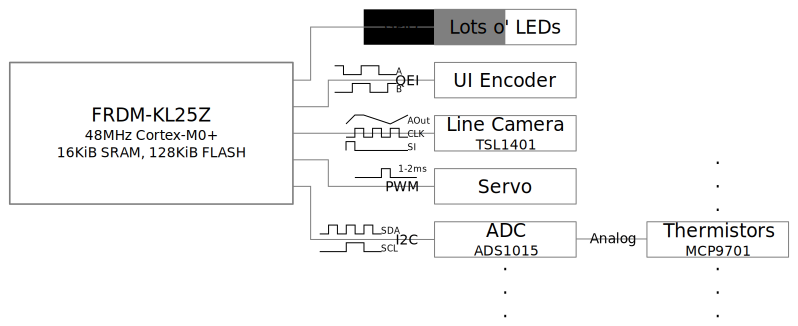
\includegraphics[width = 0.8\columnwidth]{images/192-block-diagram}
\end{figure}

\only<1> {
EECS192 course project: line-following robot car
\begin{itemize}
  \item Optical linescan camera, servo actuated steering
  \item Compute and control handled by microcontroller
  \item Lots of non-stock peripherals to bring up
\end{itemize}
}
\only<2-> {
What would be a logical way to bring up this system?
\visible<3-> {
\begin{itemize}
  \item Write hardware drivers (encoder, camera, ...)
  \item Debug hardware drivers, in combination with hardware
  \item Write application logic (line detect, control loops, ...)
\end{itemize}
}
}
\end{frame}

%---------------------------------------------------------------------
\section{Demonstration} % [?? mins]
%---------------------------------------------------------------------
\begin{frame}[fragile]
\frametitle{Sanity Check}
\begin{columns}[t]
\column{0.646\textwidth}
  What's the first thing we should bring up?
  \hfill \break
  \hfill \break
  \visible<2-> {
  Basic system test and debugging tools
  }
  \visible<3-> {
  \begin{itemize}
      \item Embedded "hello, world": blinking LEDs
      \item \texttt{printf} serial console
  \end{itemize}
  }
\column{0.323\textwidth}
  \begin{figure}
    \centering
    {\tiny
      \lstset{language=C++}
      \begin{lstlisting}
      #include "mbed.h"

      int main() {
      
      }
      \end{lstlisting}
    }
    you start here
  \end{figure}
\end{columns}
\end{frame}

\begin{frame}
\centering \huge Demonstration
\end{frame}

\begin{frame}
\frametitle{Quad Encoder}
\begin{columns}[t]
\column{0.5\textwidth}
  A quad encoder uses two digital lines to count pulses with directionality \\
  \hfill \break
  How should we code this up?
  \visible<2-> {
  \begin{itemize}
    \item Find a library online, don't reinvent the wheel {\tiny without a good reason}
    \item Someone else has written it, and many more people have tested it
  \end{itemize}
  \centering
  \includegraphics[width = 0.9\columnwidth]{external/mbed-qei-api} \\
  mbed QEI API \\
  }
\column{0.5\textwidth}
  \begin{figure}
    \centering
    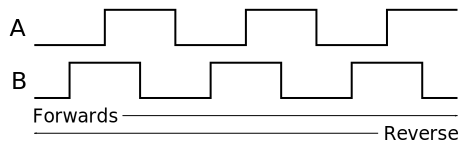
\includegraphics[width = 0.9\columnwidth]{images/quad-encoder} \\
    Quad encoder waveforms \\

  \end{figure}
\end{columns}
\end{frame}

\begin{frame}
\centering \huge Make the clicky knob work!
\end{frame}

\begin{frame}
\frametitle{Line Camera}
\begin{columns}[t]
\column{0.5\textwidth}
  Many peripherals use standard interfaces, like I2C and SPI \\
  \hfill \break
  Some don't, like this line camera
  \begin{itemize}
    \item Generally simple protocols
    \item Datasheet gives all the details
    \item Pixel data on analog line
    \item Clock signal shifts out next pixel
  \end{itemize}
\column{0.5\textwidth}
  \begin{figure}
    \centering
    \includegraphics[width = 0.9\columnwidth]{external/tsl1401-p5-waveforms} \\
    TSL1401 Datasheet, page 5
  \end{figure}
\end{columns}
\end{frame}

\begin{frame}
\centering \huge Let's write some code!
\end{frame}

\begin{frame}
\centering {\huge Now bring up the servo!} \\
\hfill \break
you've already learned the servo PWM protocol
\end{frame}

\begin{frame}
\frametitle{External ADC}
\begin{columns}[t]
\column{0.5\textwidth}
  A thermistor is connected to an external ADC, connected by I2C \\
  \hfill \break
  So let's bring up the ADC
  \begin{itemize}
    \item Datasheet describes protocol in terms of I2C transactions
    \item Basically: write configuration registers, read conversion result
  \end{itemize}
\column{0.5\textwidth}
  \begin{figure}
    \centering
    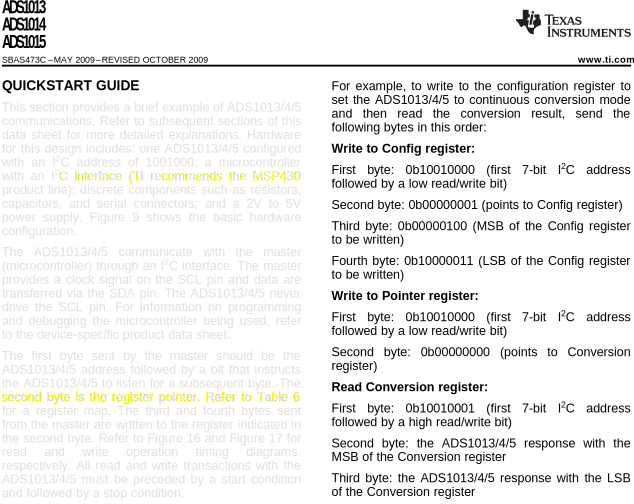
\includegraphics[width = 0.9\columnwidth]{external/ads1015-p8-writeprocedure} \\
    ADS1015 Datasheet, page 8 \\

  \end{figure}
\end{columns}
\end{frame}

\begin{frame}
\centering \huge I2C Fun Time!
\end{frame}

\begin{frame}
\frametitle{Thermistors}
\begin{columns}[t]
\column{0.5\textwidth}
  MCP9701 is a linear active thermistor
  \begin{itemize}
    \item Voltage is proportional to temperature
    \item Details (offset and scale constants) in datasheet
    \item Around 20C, what is the expected voltage?
    \visible<2->{
    \begin{itemize}
      \item ~0.8 V
    \end{itemize}
    }
    \visible<3->{
    \item How would you code up the conversion from voltage to temperature?
    }
  \end{itemize}
\column{0.5\textwidth}
  \begin{figure}
    \centering
    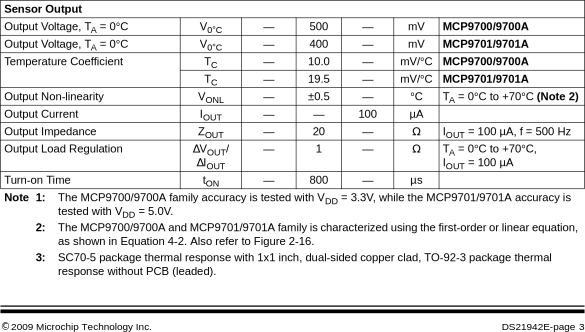
\includegraphics[width = 0.9\columnwidth]{external/mcp9701-p3-outputtable} \\
    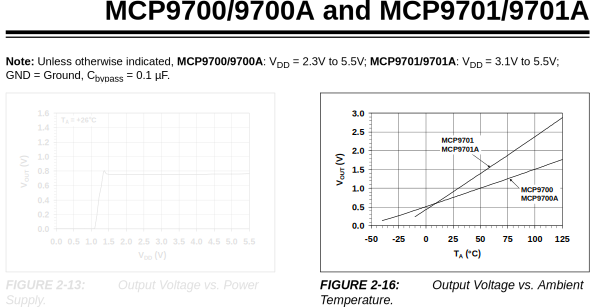
\includegraphics[width = 0.9\columnwidth]{external/mcp9701-p7-outputchart} \\
    MCP9701 Datasheet, pages 3 and 7
  \end{figure}
\end{columns}
\end{frame}

\begin{frame}
\centering {\huge Closed-loop tracking demo} \\
\hfill \break
Bringing it all together
\end{frame}

%---------------------------------------------------------------------
\section{Summary} % [?? mins]
%---------------------------------------------------------------------

\begin{frame}
\frametitle{Summary}
\begin{itemize}
  \item Whirlwind tour of embedded system bring-up with custom peripherals
  \begin{itemize}
    \item A lot of artificial failures as examples of common failure modes
    \item ... and a lot of details glossed over
  \end{itemize}
  \item Write code incrementally
  \begin{itemize}
    \item Less things added, less things to question if something goes wrong
    \item Verify each part before building on top of it
  \end{itemize}
  \item When stuff goes wrong, get visibility into the system
  \begin{itemize}
    \item \texttt{printf} for software visibility
    \item Multimeter for non-time-varying quantities, like power rails
    \item Oscilloscope for analog signals
    \item Logic analyzer for digital signals, with protocol analyzers
  \end{itemize}  
  \item Design for Test
  \begin{itemize}
    \item Make system visibility \textit{easy}, like with probe points
  \end{itemize}  
\end{itemize}
\end{frame}

\end{document}
